\PassOptionsToPackage{unicode=true}{hyperref} % options for packages loaded elsewhere
\PassOptionsToPackage{hyphens}{url}
%
\documentclass[]{article}
\usepackage{lmodern}
\usepackage{amssymb,amsmath}
\usepackage{ifxetex,ifluatex}
\usepackage{fixltx2e} % provides \textsubscript
\ifnum 0\ifxetex 1\fi\ifluatex 1\fi=0 % if pdftex
  \usepackage[T1]{fontenc}
  \usepackage[utf8]{inputenc}
  \usepackage{textcomp} % provides euro and other symbols
\else % if luatex or xelatex
  \usepackage{unicode-math}
  \defaultfontfeatures{Ligatures=TeX,Scale=MatchLowercase}
\fi
% use upquote if available, for straight quotes in verbatim environments
\IfFileExists{upquote.sty}{\usepackage{upquote}}{}
% use microtype if available
\IfFileExists{microtype.sty}{%
\usepackage[]{microtype}
\UseMicrotypeSet[protrusion]{basicmath} % disable protrusion for tt fonts
}{}
\IfFileExists{parskip.sty}{%
\usepackage{parskip}
}{% else
\setlength{\parindent}{0pt}
\setlength{\parskip}{6pt plus 2pt minus 1pt}
}
\usepackage{hyperref}
\hypersetup{
            pdftitle={Art and Artists},
            pdfauthor={Hannah Mandell},
            pdfborder={0 0 0},
            breaklinks=true}
\urlstyle{same}  % don't use monospace font for urls
\usepackage[margin=1in]{geometry}
\usepackage{color}
\usepackage{fancyvrb}
\newcommand{\VerbBar}{|}
\newcommand{\VERB}{\Verb[commandchars=\\\{\}]}
\DefineVerbatimEnvironment{Highlighting}{Verbatim}{commandchars=\\\{\}}
% Add ',fontsize=\small' for more characters per line
\usepackage{framed}
\definecolor{shadecolor}{RGB}{248,248,248}
\newenvironment{Shaded}{\begin{snugshade}}{\end{snugshade}}
\newcommand{\AlertTok}[1]{\textcolor[rgb]{0.94,0.16,0.16}{#1}}
\newcommand{\AnnotationTok}[1]{\textcolor[rgb]{0.56,0.35,0.01}{\textbf{\textit{#1}}}}
\newcommand{\AttributeTok}[1]{\textcolor[rgb]{0.77,0.63,0.00}{#1}}
\newcommand{\BaseNTok}[1]{\textcolor[rgb]{0.00,0.00,0.81}{#1}}
\newcommand{\BuiltInTok}[1]{#1}
\newcommand{\CharTok}[1]{\textcolor[rgb]{0.31,0.60,0.02}{#1}}
\newcommand{\CommentTok}[1]{\textcolor[rgb]{0.56,0.35,0.01}{\textit{#1}}}
\newcommand{\CommentVarTok}[1]{\textcolor[rgb]{0.56,0.35,0.01}{\textbf{\textit{#1}}}}
\newcommand{\ConstantTok}[1]{\textcolor[rgb]{0.00,0.00,0.00}{#1}}
\newcommand{\ControlFlowTok}[1]{\textcolor[rgb]{0.13,0.29,0.53}{\textbf{#1}}}
\newcommand{\DataTypeTok}[1]{\textcolor[rgb]{0.13,0.29,0.53}{#1}}
\newcommand{\DecValTok}[1]{\textcolor[rgb]{0.00,0.00,0.81}{#1}}
\newcommand{\DocumentationTok}[1]{\textcolor[rgb]{0.56,0.35,0.01}{\textbf{\textit{#1}}}}
\newcommand{\ErrorTok}[1]{\textcolor[rgb]{0.64,0.00,0.00}{\textbf{#1}}}
\newcommand{\ExtensionTok}[1]{#1}
\newcommand{\FloatTok}[1]{\textcolor[rgb]{0.00,0.00,0.81}{#1}}
\newcommand{\FunctionTok}[1]{\textcolor[rgb]{0.00,0.00,0.00}{#1}}
\newcommand{\ImportTok}[1]{#1}
\newcommand{\InformationTok}[1]{\textcolor[rgb]{0.56,0.35,0.01}{\textbf{\textit{#1}}}}
\newcommand{\KeywordTok}[1]{\textcolor[rgb]{0.13,0.29,0.53}{\textbf{#1}}}
\newcommand{\NormalTok}[1]{#1}
\newcommand{\OperatorTok}[1]{\textcolor[rgb]{0.81,0.36,0.00}{\textbf{#1}}}
\newcommand{\OtherTok}[1]{\textcolor[rgb]{0.56,0.35,0.01}{#1}}
\newcommand{\PreprocessorTok}[1]{\textcolor[rgb]{0.56,0.35,0.01}{\textit{#1}}}
\newcommand{\RegionMarkerTok}[1]{#1}
\newcommand{\SpecialCharTok}[1]{\textcolor[rgb]{0.00,0.00,0.00}{#1}}
\newcommand{\SpecialStringTok}[1]{\textcolor[rgb]{0.31,0.60,0.02}{#1}}
\newcommand{\StringTok}[1]{\textcolor[rgb]{0.31,0.60,0.02}{#1}}
\newcommand{\VariableTok}[1]{\textcolor[rgb]{0.00,0.00,0.00}{#1}}
\newcommand{\VerbatimStringTok}[1]{\textcolor[rgb]{0.31,0.60,0.02}{#1}}
\newcommand{\WarningTok}[1]{\textcolor[rgb]{0.56,0.35,0.01}{\textbf{\textit{#1}}}}
\usepackage{graphicx,grffile}
\makeatletter
\def\maxwidth{\ifdim\Gin@nat@width>\linewidth\linewidth\else\Gin@nat@width\fi}
\def\maxheight{\ifdim\Gin@nat@height>\textheight\textheight\else\Gin@nat@height\fi}
\makeatother
% Scale images if necessary, so that they will not overflow the page
% margins by default, and it is still possible to overwrite the defaults
% using explicit options in \includegraphics[width, height, ...]{}
\setkeys{Gin}{width=\maxwidth,height=\maxheight,keepaspectratio}
\setlength{\emergencystretch}{3em}  % prevent overfull lines
\providecommand{\tightlist}{%
  \setlength{\itemsep}{0pt}\setlength{\parskip}{0pt}}
\setcounter{secnumdepth}{0}
% Redefines (sub)paragraphs to behave more like sections
\ifx\paragraph\undefined\else
\let\oldparagraph\paragraph
\renewcommand{\paragraph}[1]{\oldparagraph{#1}\mbox{}}
\fi
\ifx\subparagraph\undefined\else
\let\oldsubparagraph\subparagraph
\renewcommand{\subparagraph}[1]{\oldsubparagraph{#1}\mbox{}}
\fi

% set default figure placement to htbp
\makeatletter
\def\fps@figure{htbp}
\makeatother


\title{Art and Artists}
\author{Hannah Mandell}
\date{1/12/2021}

\begin{document}
\maketitle

The data today come from the Tate Art Gallery
(\url{https://github.com/tategallery/collection})

\begin{Shaded}
\begin{Highlighting}[]
\KeywordTok{library}\NormalTok{(tidyverse)}
\end{Highlighting}
\end{Shaded}

\begin{verbatim}
## -- Attaching packages --------------------------------------- tidyverse 1.3.0 --
\end{verbatim}

\begin{verbatim}
## v ggplot2 3.3.2     v purrr   0.3.4
## v tibble  3.0.4     v dplyr   1.0.2
## v tidyr   1.1.2     v stringr 1.4.0
## v readr   1.3.1     v forcats 0.4.0
\end{verbatim}

\begin{verbatim}
## Warning: package 'ggplot2' was built under R version 3.6.2
\end{verbatim}

\begin{verbatim}
## Warning: package 'tibble' was built under R version 3.6.2
\end{verbatim}

\begin{verbatim}
## Warning: package 'tidyr' was built under R version 3.6.2
\end{verbatim}

\begin{verbatim}
## Warning: package 'purrr' was built under R version 3.6.2
\end{verbatim}

\begin{verbatim}
## Warning: package 'dplyr' was built under R version 3.6.2
\end{verbatim}

\begin{verbatim}
## -- Conflicts ------------------------------------------ tidyverse_conflicts() --
## x dplyr::filter() masks stats::filter()
## x dplyr::lag()    masks stats::lag()
\end{verbatim}

\begin{Shaded}
\begin{Highlighting}[]
\KeywordTok{library}\NormalTok{(tidytuesdayR)}
\end{Highlighting}
\end{Shaded}

\begin{verbatim}
## Warning: package 'tidytuesdayR' was built under R version 3.6.2
\end{verbatim}

\begin{Shaded}
\begin{Highlighting}[]
\KeywordTok{library}\NormalTok{(lubridate)}
\end{Highlighting}
\end{Shaded}

\begin{verbatim}
## 
## Attaching package: 'lubridate'
\end{verbatim}

\begin{verbatim}
## The following object is masked from 'package:base':
## 
##     date
\end{verbatim}

\begin{Shaded}
\begin{Highlighting}[]
\KeywordTok{library}\NormalTok{(dplyr)}
\KeywordTok{library}\NormalTok{(tidyr)}
\KeywordTok{library}\NormalTok{(broom)}
\end{Highlighting}
\end{Shaded}

\begin{verbatim}
## Warning: package 'broom' was built under R version 3.6.2
\end{verbatim}

\begin{Shaded}
\begin{Highlighting}[]
\KeywordTok{library}\NormalTok{(countrycode)}
\end{Highlighting}
\end{Shaded}

\begin{verbatim}
## Warning: package 'countrycode' was built under R version 3.6.2
\end{verbatim}

\begin{Shaded}
\begin{Highlighting}[]
\KeywordTok{library}\NormalTok{(praise)}
\CommentTok{#install.packages("tidymodels")}
\KeywordTok{library}\NormalTok{(tidymodels)}
\end{Highlighting}
\end{Shaded}

\begin{verbatim}
## Warning: package 'tidymodels' was built under R version 3.6.2
\end{verbatim}

\begin{verbatim}
## -- Attaching packages -------------------------------------- tidymodels 0.1.2 --
\end{verbatim}

\begin{verbatim}
## v dials     0.0.9      v rsample   0.0.8 
## v infer     0.5.3      v tune      0.1.2 
## v modeldata 0.1.0      v workflows 0.2.1 
## v parsnip   0.1.4      v yardstick 0.0.7 
## v recipes   0.1.15
\end{verbatim}

\begin{verbatim}
## Warning: package 'dials' was built under R version 3.6.2
\end{verbatim}

\begin{verbatim}
## Warning: package 'infer' was built under R version 3.6.2
\end{verbatim}

\begin{verbatim}
## Warning: package 'modeldata' was built under R version 3.6.2
\end{verbatim}

\begin{verbatim}
## Warning: package 'parsnip' was built under R version 3.6.2
\end{verbatim}

\begin{verbatim}
## Warning: package 'recipes' was built under R version 3.6.2
\end{verbatim}

\begin{verbatim}
## Warning: package 'rsample' was built under R version 3.6.2
\end{verbatim}

\begin{verbatim}
## Warning: package 'tune' was built under R version 3.6.2
\end{verbatim}

\begin{verbatim}
## Warning: package 'workflows' was built under R version 3.6.2
\end{verbatim}

\begin{verbatim}
## Warning: package 'yardstick' was built under R version 3.6.2
\end{verbatim}

\begin{verbatim}
## -- Conflicts ----------------------------------------- tidymodels_conflicts() --
## x scales::discard() masks purrr::discard()
## x dplyr::filter()   masks stats::filter()
## x recipes::fixed()  masks stringr::fixed()
## x dplyr::lag()      masks stats::lag()
## x yardstick::spec() masks readr::spec()
## x recipes::step()   masks stats::step()
\end{verbatim}

\begin{Shaded}
\begin{Highlighting}[]
\CommentTok{#install.packages("ranger")}
\end{Highlighting}
\end{Shaded}

\begin{Shaded}
\begin{Highlighting}[]
\KeywordTok{praise}\NormalTok{()}
\end{Highlighting}
\end{Shaded}

\begin{verbatim}
## [1] "You are spectacular!"
\end{verbatim}

\hypertarget{get-the-data}{%
\section{Get the Data}\label{get-the-data}}

\begin{Shaded}
\begin{Highlighting}[]
\NormalTok{tt_data <-}\StringTok{ }\KeywordTok{tt_load}\NormalTok{(}\StringTok{"2021-01-12"}\NormalTok{)}
\end{Highlighting}
\end{Shaded}

\begin{verbatim}
## --- Compiling #TidyTuesday Information for 2021-01-12 ----
\end{verbatim}

\begin{verbatim}
## --- There are 2 files available ---
\end{verbatim}

\begin{verbatim}
## --- Starting Download ---
\end{verbatim}

\begin{verbatim}
## 
##  Downloading file 1 of 2: `artists.csv`
##  Downloading file 2 of 2: `artwork.csv`
\end{verbatim}

\begin{verbatim}
## --- Download complete ---
\end{verbatim}

\begin{Shaded}
\begin{Highlighting}[]
\CommentTok{# make and save csvs}
\NormalTok{artwork <-}\StringTok{ }\NormalTok{tt_data}\OperatorTok{$}\NormalTok{artwork}
\KeywordTok{write_csv}\NormalTok{(artwork, }\StringTok{"artwork.csv"}\NormalTok{)}
\NormalTok{artists <-}\StringTok{ }\NormalTok{tt_data}\OperatorTok{$}\NormalTok{artists}
\KeywordTok{write_csv}\NormalTok{(artists, }\StringTok{"artists.csv"}\NormalTok{)}
\end{Highlighting}
\end{Shaded}

\hypertarget{preliminary-looks-at-the-data}{%
\section{Preliminary looks at the
data}\label{preliminary-looks-at-the-data}}

\begin{Shaded}
\begin{Highlighting}[]
\KeywordTok{head}\NormalTok{(artwork)}
\end{Highlighting}
\end{Shaded}

\begin{verbatim}
## # A tibble: 6 x 20
##      id accession_number artist artistRole artistId title dateText medium
##   <dbl> <chr>            <chr>  <chr>         <dbl> <chr> <chr>    <chr> 
## 1  1035 A00001           Blake~ artist           38 A Fi~ date no~ Water~
## 2  1036 A00002           Blake~ artist           38 Two ~ date no~ Graph~
## 3  1037 A00003           Blake~ artist           38 The ~ ?c.1785  Graph~
## 4  1038 A00004           Blake~ artist           38 Six ~ date no~ Graph~
## 5  1039 A00005           Blake~ artist           39 The ~ 1826–7,~ Line ~
## 6  1040 A00006           Blake~ artist           39 Ciam~ 1826–7,~ Line ~
## # ... with 12 more variables: creditLine <chr>, year <dbl>,
## #   acquisitionYear <dbl>, dimensions <chr>, width <dbl>, height <dbl>,
## #   depth <dbl>, units <chr>, inscription <chr>, thumbnailCopyright <lgl>,
## #   thumbnailUrl <chr>, url <chr>
\end{verbatim}

\begin{Shaded}
\begin{Highlighting}[]
\KeywordTok{glimpse}\NormalTok{(artwork)}
\end{Highlighting}
\end{Shaded}

\begin{verbatim}
## Rows: 69,201
## Columns: 20
## $ id                 <dbl> 1035, 1036, 1037, 1038, 1039, 1040, 1041, 1042, ...
## $ accession_number   <chr> "A00001", "A00002", "A00003", "A00004", "A00005"...
## $ artist             <chr> "Blake, Robert", "Blake, Robert", "Blake, Robert...
## $ artistRole         <chr> "artist", "artist", "artist", "artist", "artist"...
## $ artistId           <dbl> 38, 38, 38, 38, 39, 39, 39, 39, 39, 39, 39, 39, ...
## $ title              <chr> "A Figure Bowing before a Seated Old Man with hi...
## $ dateText           <chr> "date not known", "date not known", "?c.1785", "...
## $ medium             <chr> "Watercolour, ink, chalk and graphite on paper. ...
## $ creditLine         <chr> "Presented by Mrs John Richmond 1922", "Presente...
## $ year               <dbl> NA, NA, 1785, NA, 1826, 1826, 1826, 1826, 1826, ...
## $ acquisitionYear    <dbl> 1922, 1922, 1922, 1922, 1919, 1919, 1919, 1919, ...
## $ dimensions         <chr> "support: 394 x 419 mm", "support: 311 x 213 mm"...
## $ width              <dbl> 394, 311, 343, 318, 243, 240, 242, 246, 241, 243...
## $ height             <dbl> 419, 213, 467, 394, 335, 338, 334, 340, 335, 340...
## $ depth              <dbl> NA, NA, NA, NA, NA, NA, NA, NA, NA, NA, NA, NA, ...
## $ units              <chr> "mm", "mm", "mm", "mm", "mm", "mm", "mm", "mm", ...
## $ inscription        <chr> NA, NA, NA, NA, NA, NA, NA, NA, NA, NA, NA, NA, ...
## $ thumbnailCopyright <lgl> NA, NA, NA, NA, NA, NA, NA, NA, NA, NA, NA, NA, ...
## $ thumbnailUrl       <chr> "http://www.tate.org.uk/art/images/work/A/A00/A0...
## $ url                <chr> "http://www.tate.org.uk/art/artworks/blake-a-fig...
\end{verbatim}

\begin{Shaded}
\begin{Highlighting}[]
\KeywordTok{head}\NormalTok{(artists)}
\end{Highlighting}
\end{Shaded}

\begin{verbatim}
## # A tibble: 6 x 9
##      id name  gender dates yearOfBirth yearOfDeath placeOfBirth placeOfDeath
##   <dbl> <chr> <chr>  <chr>       <dbl>       <dbl> <chr>        <chr>       
## 1 10093 Abak~ Female born~        1930          NA Polska       <NA>        
## 2     0 Abbe~ Male   1852~        1852        1911 Philadelphi~ London, Uni~
## 3  2756 Abbo~ Female 1898~        1898        1991 Springfield~ Monson, Uni~
## 4     1 Abbo~ Male   1760~        1760        1803 Leicestersh~ London, Uni~
## 5   622 Abra~ Male   born~        1935          NA Wigan, Unit~ <NA>        
## 6  2606 Absa~ Male   1964~        1964        1993 Tel Aviv-Ya~ Paris, Fran~
## # ... with 1 more variable: url <chr>
\end{verbatim}

\begin{Shaded}
\begin{Highlighting}[]
\KeywordTok{glimpse}\NormalTok{(artists)}
\end{Highlighting}
\end{Shaded}

\begin{verbatim}
## Rows: 3,532
## Columns: 9
## $ id           <dbl> 10093, 0, 2756, 1, 622, 2606, 9550, 623, 624, 625, 241...
## $ name         <chr> "Abakanowicz, Magdalena", "Abbey, Edwin Austin", "Abbo...
## $ gender       <chr> "Female", "Male", "Female", "Male", "Male", "Male", "F...
## $ dates        <chr> "born 1930", "1852–1911", "1898–1991", "1760–1803", "b...
## $ yearOfBirth  <dbl> 1930, 1852, 1898, 1760, 1935, 1964, 1967, 1940, 1947, ...
## $ yearOfDeath  <dbl> NA, 1911, 1991, 1803, NA, 1993, NA, NA, 2014, NA, 1792...
## $ placeOfBirth <chr> "Polska", "Philadelphia, United States", "Springfield,...
## $ placeOfDeath <chr> NA, "London, United Kingdom", "Monson, United States",...
## $ url          <chr> "http://www.tate.org.uk/art/artists/magdalena-abakanow...
\end{verbatim}

Note: over half of the pieces are by Joseph Turner! We might be
interested in analyzing the data without his work.

\begin{Shaded}
\begin{Highlighting}[]
\NormalTok{artwork }\OperatorTok
\StringTok{  }\KeywordTok{group_by}\NormalTok{(artistId) }\OperatorTok
\StringTok{  }\KeywordTok{summarize}\NormalTok{(}\DataTypeTok{count =} \KeywordTok{n}\NormalTok{()) }\OperatorTok
\StringTok{  }\KeywordTok{arrange}\NormalTok{(}\KeywordTok{desc}\NormalTok{(count)) }\OperatorTok
\StringTok{  }\KeywordTok{head}\NormalTok{()}
\end{Highlighting}
\end{Shaded}

\begin{verbatim}
## `summarise()` ungrouping output (override with `.groups` argument)
\end{verbatim}

\begin{verbatim}
## # A tibble: 6 x 2
##   artistId count
##      <dbl> <int>
## 1      558 39389
## 2      300  1046
## 3     1659   623
## 4      138   612
## 5      747   578
## 6     2638   388
\end{verbatim}

\begin{Shaded}
\begin{Highlighting}[]
\NormalTok{artists }\OperatorTok
\StringTok{  }\KeywordTok{filter}\NormalTok{(id }\OperatorTok{==}\StringTok{ }\DecValTok{558}\NormalTok{)}
\end{Highlighting}
\end{Shaded}

\begin{verbatim}
## # A tibble: 1 x 9
##      id name  gender dates yearOfBirth yearOfDeath placeOfBirth placeOfDeath
##   <dbl> <chr> <chr>  <chr>       <dbl>       <dbl> <chr>        <chr>       
## 1   558 Turn~ Male   1775~        1775        1851 London, Uni~ Chelsea, Un~
## # ... with 1 more variable: url <chr>
\end{verbatim}

Both \texttt{placeofBirth} and \texttt{placeofDeath} are given as City,
Country. Let's look to split these into different categories - it might
make it easier to analyze or model the data.

\begin{Shaded}
\begin{Highlighting}[]
\NormalTok{artists <-}\StringTok{ }\NormalTok{artists }\OperatorTok
\StringTok{  }\KeywordTok{separate}\NormalTok{(placeOfBirth, }\KeywordTok{c}\NormalTok{(}\StringTok{"cityBirth"}\NormalTok{, }\StringTok{"countryBirth"}\NormalTok{), }\DataTypeTok{sep =} \StringTok{", "}\NormalTok{, }\DataTypeTok{fill =} \StringTok{"left"}\NormalTok{) }\OperatorTok
\StringTok{  }\KeywordTok{separate}\NormalTok{(placeOfDeath, }\KeywordTok{c}\NormalTok{(}\StringTok{"cityDeath"}\NormalTok{, }\StringTok{"countryDeath"}\NormalTok{), }\DataTypeTok{sep =} \StringTok{", "}\NormalTok{, }\DataTypeTok{fill =} \StringTok{"left"}\NormalTok{)}
\end{Highlighting}
\end{Shaded}

\begin{verbatim}
## Warning: Expected 2 pieces. Additional pieces discarded in 6 rows [530, 580,
## 1166, 1167, 1791, 2485].
\end{verbatim}

\begin{verbatim}
## Warning: Expected 2 pieces. Additional pieces discarded in 6 rows [92, 326, 545,
## 1059, 1959, 3314].
\end{verbatim}

\begin{Shaded}
\begin{Highlighting}[]
\NormalTok{artists }\OperatorTok\StringTok{ }\KeywordTok{select}\NormalTok{(countryBirth) }\OperatorTok\StringTok{ }\KeywordTok{table}\NormalTok{()}
\end{Highlighting}
\end{Shaded}

\begin{verbatim}
## .
##                           Al-‘Iraq                         Al-Jaza'ir 
##                                  1                                  2 
##                          Al-Lubnan                          Argentina 
##                                  8                                 17 
##                            Armenia                           As-Sudan 
##                                  1                                  1 
##                          Australia                            Auteuil 
##                                 23                                  1 
##                            Bahamas                         Bangladesh 
##                                  1                                  2 
##                           Barbados                         Beckington 
##                                  1                                  1 
##                            Belarus                             België 
##                                  4                                 37 
##                              Bénin                         Bermondsey 
##                                  1                                  1 
##                             Bharat                         Blackheath 
##                                 24                                  1 
##                Bosna i Hercegovina                          Braintree 
##                                  2                                  1 
##                             Brasil                            Bristol 
##                                 30                                  2 
##                           Bulgaria                           Cameroun 
##                                  2                                  1 
##                             Canada                         Canterbury 
##                                 40                                  1 
##                    Ceská Republika                           Charlieu 
##                                 14                                  1 
##                   Charlotte Amalie                              Chile 
##                                  1                                  5 
## Choson Minjujuui In'min Konghwaguk                  Chung-hua Min-kuo 
##                                  1                                  1 
##                           Colombia                         Costa Rica 
##                                  8                                  1 
##                               Cuba                               D.C. 
##                                  9                                  2 
##                            Danmark                  Département de la 
##                                  9                                  1 
##                        Deutschland                            Douglas 
##                                142                                  1 
##                          Edinburgh                              Eesti 
##                                  1                                  1 
##                           Egremont                               Éire 
##                                  1                                 51 
##                              Ellás                              Epsom 
##                                 10                                  1 
##                             España                             France 
##                                 29                                157 
##                             Guyana                      Hertfordshire 
##                                  2                                  1 
##                           Hrvatska                          Indonesia 
##                                  8                                  2 
##                               Îran                             Ísland 
##                                 10                                  1 
##                        Isle of Man                             Italia 
##                                  2                                 80 
##                            Jamaica                        Jugoslavija 
##                                  2                                  3 
##                         Kensington                              Kenya 
##                                  1                                  1 
##                                Lao                            Latvija 
##                                  1                                  3 
##                            Lietuva                          Liverpool 
##                                  4                                  1 
##                             London                         Luxembourg 
##                                  3                                  1 
##                       Magyarország                         Makedonija 
##                                 13                                  1 
##                           Malaysia                              Malta 
##                                  1                                  1 
##                          Mauritius                              Mehoz 
##                                  2                                  2 
##                           Melmerby                             México 
##                                  1                                 13 
##                               Misr                            Moldova 
##                                  8                                  1 
##                         Montserrat                            Myanmar 
##                                  1                                  1 
##                          Nederland                        New Zealand 
##                                 35                                 10 
##                          Nicaragua                    Niederschlesien 
##                                  1                                  1 
##                            Nigeria                              Nihon 
##                                  1                                 27 
##                              Norge                         Österreich 
##                                  3                                 29 
##                               Otok                           Pakistan 
##                                  1                                  5 
##                             Panamá                              Perth 
##                                  1                                  1 
##                               Perú                          Pilipinas 
##                                  4                                  1 
##                           Plymouth                             Polska 
##                                  1                                 41 
##                           Portugal                       Prathet Thai 
##                                 10                                  1 
##                           Rochdale                            România 
##                                  1                                 13 
##                            Rossiya                       Saint Hélier 
##                                 32                                  2 
##                              Samoa                          Schlesien 
##                                  1                                  2 
##                            Schweiz                          Shqipëria 
##                                 29                                  1 
##                          Singapore                          Slovenija 
##                                  2                                  6 
##                Slovenská Republika                          Solothurn 
##                                  3                                  1 
##                       South Africa                          Sri Lanka 
##                                 20                                  3 
##                      Staten Island                          Stockholm 
##                                  1                                  1 
##                     Stoke on Trent                              Suomi 
##                                  1                                  1 
##                            Suriyah                            Sverige 
##                                  2                                 12 
##                     Taehan Min'guk                           Tanzania 
##                                  3                                  1 
##                              Tunis                            Türkiye 
##                                  1                                  6 
##                             Uganda                           Ukrayina 
##                                  1                                 17 
##                     United Kingdom                      United States 
##                               1496                                339 
##                          Venezuela                           Viet Nam 
##                                  7                                  2 
##                          Wimbledon                           Yisra'el 
##                                  1                                 11 
##                             Zambia                           Zhonghua 
##                                  1                                 22 
##                           Zimbabwe 
##                                  1
\end{verbatim}

\begin{Shaded}
\begin{Highlighting}[]
\NormalTok{artists }\OperatorTok
\StringTok{  }\KeywordTok{group_by}\NormalTok{(countryBirth) }\OperatorTok
\StringTok{  }\KeywordTok{mutate}\NormalTok{(}\DataTypeTok{count =} \KeywordTok{n}\NormalTok{()) }\OperatorTok
\StringTok{  }\KeywordTok{filter}\NormalTok{(count }\OperatorTok{>=}\StringTok{ }\DecValTok{10}\NormalTok{) }\OperatorTok
\StringTok{  }\KeywordTok{ungroup}\NormalTok{() }\OperatorTok
\StringTok{  }\KeywordTok{ggplot}\NormalTok{(}\KeywordTok{aes}\NormalTok{(}\DataTypeTok{x =}\NormalTok{ countryBirth, }\DataTypeTok{y =}\NormalTok{ yearOfBirth)) }\OperatorTok{+}
\StringTok{  }\KeywordTok{geom_boxplot}\NormalTok{()}
\end{Highlighting}
\end{Shaded}

\begin{verbatim}
## Warning: Removed 60 rows containing non-finite values (stat_boxplot).
\end{verbatim}

\includegraphics{art_files/figure-latex/boxplot of country \& year of artwork-1.pdf}

\hypertarget{joins}{%
\section{Joins!}\label{joins}}

Combining datasets with shared unique identifiers: Inner Join = keep
everything that is shared in both datasets Full Union = keep everything
from each dataset

Let's combine the datasets so that if we want to use gender to ask
questions about the art, the information is available!

\begin{Shaded}
\begin{Highlighting}[]
\NormalTok{artartist1 <-}\StringTok{ }
\StringTok{  }\KeywordTok{inner_join}\NormalTok{(artists, artwork, }\DataTypeTok{by =} \KeywordTok{c}\NormalTok{(}\StringTok{"id"}\NormalTok{ =}\StringTok{ "artistId"}\NormalTok{))}

\NormalTok{artartist2 <-}\StringTok{ }
\StringTok{  }\KeywordTok{full_join}\NormalTok{(artists, artwork, }\DataTypeTok{by =} \KeywordTok{c}\NormalTok{(}\StringTok{"id"}\NormalTok{ =}\StringTok{ "artistId"}\NormalTok{))}

\KeywordTok{nrow}\NormalTok{(artwork)}
\end{Highlighting}
\end{Shaded}

\begin{verbatim}
## [1] 69201
\end{verbatim}

\begin{Shaded}
\begin{Highlighting}[]
\KeywordTok{nrow}\NormalTok{(artartist1)}
\end{Highlighting}
\end{Shaded}

\begin{verbatim}
## [1] 69195
\end{verbatim}

\begin{Shaded}
\begin{Highlighting}[]
\KeywordTok{nrow}\NormalTok{(artartist2)}
\end{Highlighting}
\end{Shaded}

\begin{verbatim}
## [1] 69395
\end{verbatim}

Some inportant insights from these runs:

There are 6 pieces of art that do not have a listed artist. They are
left out in the intersect.

There are ALSO 194 artists in the dataset that do not have artwork in
the database, and that is why we get MORE data in artartist2 than in
artwork itself.

\hypertarget{visualization}{%
\section{Visualization}\label{visualization}}

\begin{Shaded}
\begin{Highlighting}[]
\NormalTok{artwork }\OperatorTok
\StringTok{  }\KeywordTok{select}\NormalTok{(artistRole) }\OperatorTok
\StringTok{  }\KeywordTok{table}\NormalTok{()}
\end{Highlighting}
\end{Shaded}

\begin{verbatim}
## .
##                    after              and a pupil           and assistants 
##                     2014                        4                        3 
##        and other artists               and studio                   artist 
##                       12                        1                    66907 
##            attributed to                circle of doubtfully attributed to 
##                      164                        1                        1 
##              follower of   formerly attributed to              imitator of 
##                        2                       14                        5 
##                manner of             prints after                   pseudo 
##                       24                       11                        8 
##                 pupil of                school of                studio of 
##                       18                        4                        7 
##                 style of 
##                        1
\end{verbatim}

\begin{Shaded}
\begin{Highlighting}[]
\CommentTok{#density plot}
\NormalTok{artartist1 }\OperatorTok
\StringTok{  }\KeywordTok{filter}\NormalTok{(id }\OperatorTok{!=}\StringTok{ }\DecValTok{558}\NormalTok{) }\OperatorTok
\StringTok{  }\KeywordTok{ggplot}\NormalTok{(}\KeywordTok{aes}\NormalTok{(}\DataTypeTok{x =}\NormalTok{ year, }\DataTypeTok{color =}\NormalTok{ gender)) }\OperatorTok{+}\StringTok{ }
\StringTok{  }\KeywordTok{geom_density}\NormalTok{()}
\end{Highlighting}
\end{Shaded}

\begin{verbatim}
## Warning: Removed 5054 rows containing non-finite values (stat_density).
\end{verbatim}

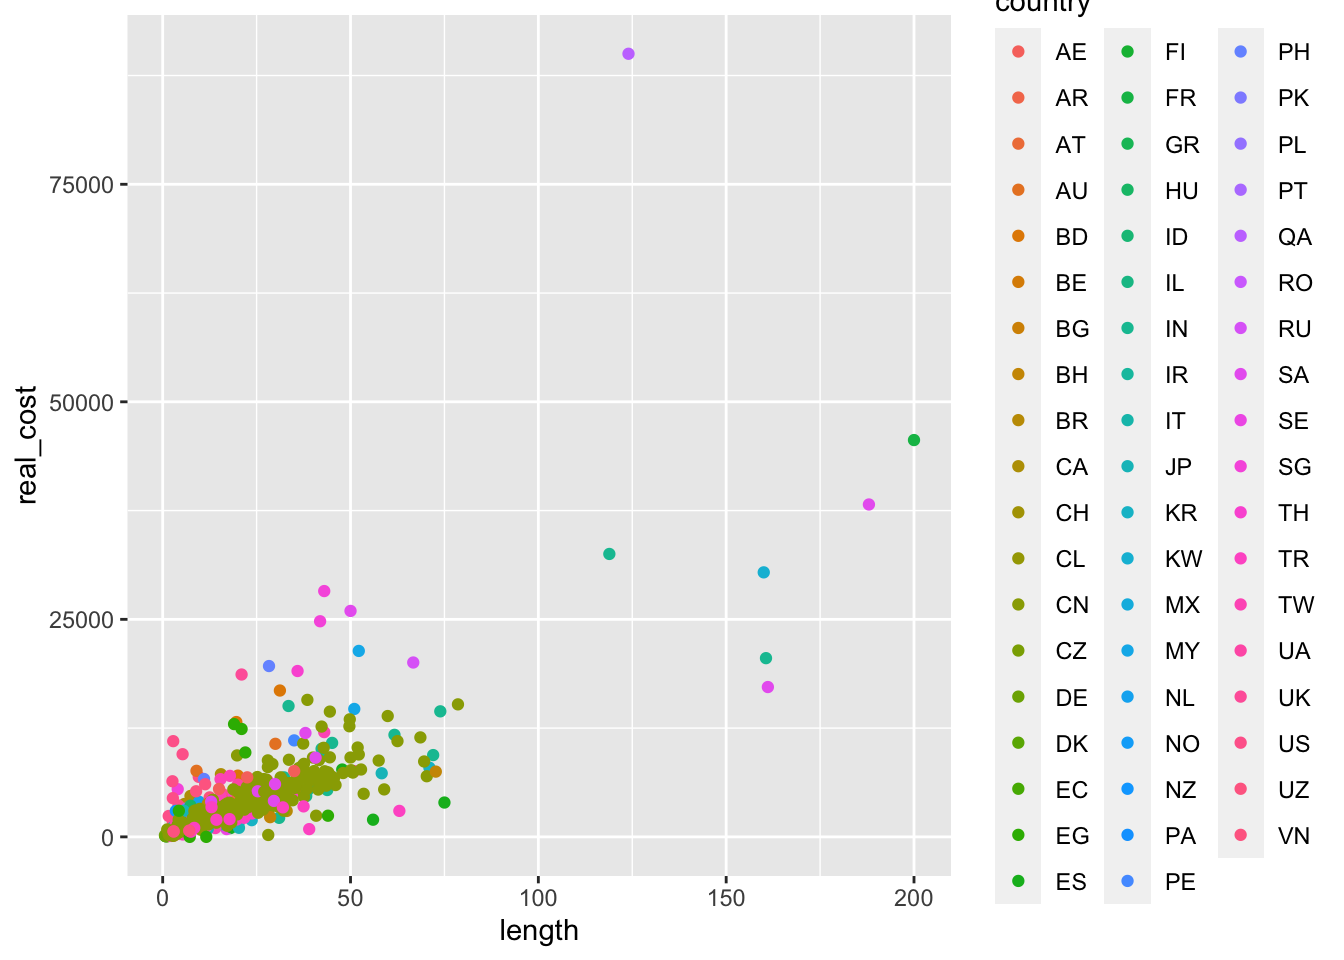
\includegraphics{art_files/figure-latex/unnamed-chunk-7-1.pdf}

\begin{Shaded}
\begin{Highlighting}[]
\CommentTok{#histogram}
\NormalTok{artartist1 }\OperatorTok
\StringTok{  }\KeywordTok{filter}\NormalTok{(id }\OperatorTok{!=}\StringTok{ }\DecValTok{558}\NormalTok{) }\OperatorTok
\StringTok{  }\KeywordTok{ggplot}\NormalTok{(}\KeywordTok{aes}\NormalTok{(}\DataTypeTok{x =}\NormalTok{ year, }\DataTypeTok{color =}\NormalTok{ gender, }\DataTypeTok{fill =}\NormalTok{ gender)) }\OperatorTok{+}\StringTok{ }
\StringTok{  }\KeywordTok{geom_histogram}\NormalTok{()}
\end{Highlighting}
\end{Shaded}

\begin{verbatim}
## `stat_bin()` using `bins = 30`. Pick better value with `binwidth`.
\end{verbatim}

\begin{verbatim}
## Warning: Removed 5054 rows containing non-finite values (stat_bin).
\end{verbatim}

\includegraphics{art_files/figure-latex/unnamed-chunk-7-2.pdf}

We see that the relative proportion of female artwork increases as we
turn towards modern times. Removing artist \# 558 helps remove his skew.

\hypertarget{random-forest-model}{%
\section{Random Forest Model}\label{random-forest-model}}

Let's explore a RFM.

\begin{Shaded}
\begin{Highlighting}[]
\KeywordTok{set.seed}\NormalTok{(}\DecValTok{47}\NormalTok{)}
\KeywordTok{library}\NormalTok{(tidymodels)}
\KeywordTok{library}\NormalTok{(vip)}
\end{Highlighting}
\end{Shaded}

\begin{verbatim}
## Warning: package 'vip' was built under R version 3.6.2
\end{verbatim}

\begin{verbatim}
## 
## Attaching package: 'vip'
\end{verbatim}

\begin{verbatim}
## The following object is masked from 'package:utils':
## 
##     vi
\end{verbatim}

\begin{Shaded}
\begin{Highlighting}[]
\CommentTok{# remove the artist that is listed an enormous number of times }
\CommentTok{# because he might skew the data}
\NormalTok{artRF <-}\StringTok{ }\NormalTok{artartist1 }\OperatorTok
\StringTok{  }\KeywordTok{filter}\NormalTok{(id }\OperatorTok{!=}\StringTok{ }\DecValTok{558}\NormalTok{)}

\CommentTok{# 75% train, 25% test}
\NormalTok{data_split <-}\StringTok{ }\KeywordTok{initial_split}\NormalTok{(artRF, }\DataTypeTok{prop =} \FloatTok{0.75}\NormalTok{)}


\NormalTok{art_train <-}\StringTok{ }\KeywordTok{training}\NormalTok{(data_split)}

\CommentTok{# for better data science, we would perform more analysis on these}
\CommentTok{# individual fields, but removing them is sufficient for our low-stakes }
\CommentTok{# purposes now}
\NormalTok{art_test  <-}\StringTok{ }\KeywordTok{testing}\NormalTok{(data_split) }\OperatorTok
\StringTok{  }\KeywordTok{filter}\NormalTok{(}\OperatorTok{!}\KeywordTok{is.na}\NormalTok{(gender)) }\OperatorTok
\StringTok{  }\KeywordTok{filter}\NormalTok{(}\OperatorTok{!}\KeywordTok{is.na}\NormalTok{(width)) }\OperatorTok
\StringTok{  }\KeywordTok{filter}\NormalTok{(}\OperatorTok{!}\KeywordTok{is.na}\NormalTok{(height)) }\OperatorTok
\StringTok{  }\KeywordTok{filter}\NormalTok{(}\OperatorTok{!}\KeywordTok{is.na}\NormalTok{(acquisitionYear)) }\OperatorTok
\StringTok{  }\KeywordTok{filter}\NormalTok{(}\OperatorTok{!}\KeywordTok{is.na}\NormalTok{(yearOfBirth)) }\OperatorTok
\StringTok{  }\KeywordTok{filter}\NormalTok{(}\OperatorTok{!}\KeywordTok{is.na}\NormalTok{(yearOfDeath))}

\CommentTok{# give it the right fields to look at}
\CommentTok{# birth and death year might make the model overfit to the training data}
\KeywordTok{rand_forest}\NormalTok{(}\DataTypeTok{mode =} \StringTok{"regression"}\NormalTok{) }\OperatorTok\StringTok{ }
\StringTok{   }\KeywordTok{set_args}\NormalTok{(}\DataTypeTok{importance =} \StringTok{"permutation"}\NormalTok{) }\OperatorTok
\StringTok{   }\KeywordTok{fit}\NormalTok{(year }\OperatorTok{~}\StringTok{ }\NormalTok{gender }\OperatorTok{+}\StringTok{ }\NormalTok{width }\OperatorTok{+}\StringTok{ }\NormalTok{height }\OperatorTok{+}\StringTok{ }\NormalTok{acquisitionYear }\OperatorTok{+}
\StringTok{         }\NormalTok{yearOfBirth }\OperatorTok{+}\StringTok{ }\NormalTok{yearOfDeath, }
       \DataTypeTok{data =}\NormalTok{ art_train) }\OperatorTok\StringTok{ }
\StringTok{   }\NormalTok{vip}\OperatorTok{::}\KeywordTok{vip}\NormalTok{() }
\end{Highlighting}
\end{Shaded}

\begin{verbatim}
## Warning: Engine set to `ranger`.
\end{verbatim}

\includegraphics{art_files/figure-latex/unnamed-chunk-8-1.pdf} We see
that the model is relying very heavily on \texttt{yearOfBirth} and
\texttt{yearOfDeath} to make its predictions, as we hypothesized.

\begin{Shaded}
\begin{Highlighting}[]
\KeywordTok{rand_forest}\NormalTok{(}\DataTypeTok{mode =} \StringTok{"regression"}\NormalTok{) }\OperatorTok\StringTok{ }
\StringTok{   }\KeywordTok{fit}\NormalTok{(year }\OperatorTok{~}\StringTok{ }\NormalTok{gender }\OperatorTok{+}\StringTok{ }\NormalTok{width }\OperatorTok{+}\StringTok{ }\NormalTok{height }\OperatorTok{+}\StringTok{ }\NormalTok{acquisitionYear }\OperatorTok{+}
\StringTok{         }\NormalTok{yearOfBirth }\OperatorTok{+}\StringTok{ }\NormalTok{yearOfDeath, }\DataTypeTok{data =}\NormalTok{ art_train) }\OperatorTok\StringTok{ }
\StringTok{   }\KeywordTok{predict}\NormalTok{(}\DataTypeTok{new_data =}\NormalTok{ art_test) }\OperatorTok
\StringTok{   }\KeywordTok{ggplot}\NormalTok{(}\KeywordTok{aes}\NormalTok{(}\DataTypeTok{y =}\NormalTok{ .pred, }\DataTypeTok{x =}\NormalTok{ art_test}\OperatorTok{$}\NormalTok{year)) }\OperatorTok{+}\StringTok{ }
\StringTok{   }\KeywordTok{geom_point}\NormalTok{() }\OperatorTok{+}
\StringTok{   }\KeywordTok{geom_abline}\NormalTok{(}\DataTypeTok{intercept =} \DecValTok{0}\NormalTok{, }\DataTypeTok{slope =} \DecValTok{1}\NormalTok{) }\OperatorTok{+}
\StringTok{  }\KeywordTok{ylab}\NormalTok{(}\StringTok{"Predicted Year"}\NormalTok{) }\OperatorTok{+}
\StringTok{  }\KeywordTok{xlab}\NormalTok{(}\StringTok{"Year of Creation"}\NormalTok{)}
\end{Highlighting}
\end{Shaded}

\begin{verbatim}
## Warning: Engine set to `ranger`.
\end{verbatim}

\begin{verbatim}
## Warning: Removed 856 rows containing missing values (geom_point).
\end{verbatim}

\includegraphics{art_files/figure-latex/unnamed-chunk-9-1.pdf} The above
graph shows that our model has a very high accuracy - probably too
accurate.

\end{document}
